\documentclass{beamer}
\usetheme{Boadilla}

%%%%%%%%%%%%%%
%% Packages %%
%%%%%%%%%%%%%%

\usepackage[export]{adjustbox}
\usepackage[absolute,overlay]{textpos}
\usepackage{mathtools}
\usepackage{amsmath}
\usepackage{listings}


\definecolor{links}{HTML}{2A1B81}
\hypersetup{colorlinks,linkcolor=,urlcolor=links}

\makeatletter
\setbeamertemplate{footline}
{
	\leavevmode%
	\hbox{%
		\begin{beamercolorbox}[wd=.333333\paperwidth,ht=2.25ex,dp=1ex,center]{author in head/foot}%
			\usebeamerfont{author in head/foot}\insertshortauthor%~~\beamer@ifempty{\insertshortinstitute}{}{(\insertshortinstitute)}
		\end{beamercolorbox}%
		\begin{beamercolorbox}[wd=.333333\paperwidth,ht=2.25ex,dp=1ex,center]{title in head/foot}%
			\usebeamerfont{title in head/foot}\insertshorttitle
		\end{beamercolorbox}%
		\begin{beamercolorbox}[wd=.333333\paperwidth,ht=2.25ex,dp=1ex,right]{date in head/foot}%
			\usebeamerfont{date in head/foot}\insertshortdate{}\hspace*{2em}
			\insertframenumber{} / \inserttotalframenumber\hspace*{2ex} 
	\end{beamercolorbox}}%
	\vskip0pt%
}
\makeatother


%%%%%%%%%%%%%%%%
%% Title Page %%
%%%%%%%%%%%%%%%%

\title[Science Incentives]{How Current Incentives for Scientists Lead to Poor Science for Everyone}
\subtitle{\textit{Everything is F*cked}}
\author{Dr. Alexander Mark Weber}
\institute{Assistant Professor, Department of Pediatrics,\\
	Division of Neurology, Faculty of Medicine\\
	Imaging Staff Scientist, BC Children's Hospital Research Institute\\
	University of British Columbia}
\date{Oct 12th, 2023}


%%%%%%%%%%%%%%
%% Document %%
%%%%%%%%%%%%%%


\begin{document}

\begin{frame}
\titlepage
\end{frame}

%%%%%%%%%%%%%%
%% Overview %%
%%%%%%%%%%%%%%

\begin{frame}{Overview}
	\tableofcontents
\end{frame}

%%%%%%%%%
%% Too %%
%%%%%%%%%

\section{Toot}
\begin{frame}{A Toot}

	\begin{columns}
		\column{0.55\textwidth}
		
\includegraphics[width=1\textwidth]{../images/Toot}

		\column{0.45\textwidth}
	\end{columns}

\end{frame}

\begin{frame}{A Toot}

	\begin{columns}
		\column{0.55\textwidth}
		
\includegraphics[width=1\textwidth]{../images/Toot_yyn}

		\column{0.45\textwidth}
		\begin{textblock*}{170pt}(190pt,45pt)
			\begin{itemize}
			\item<2-> Katalin Kariko - won for mRNA/COVID research; previously demoted from U of Pennsylvania
			\item<3-> Stanford President (Marc Tessier-Lavigne) authored 12 reports that contained false information; Harvard Professor Francesca Gino found to have manually adjusted data in at least four papers
			\item<4-> \textbf{``We have to stop rewarding short term flashy work and overproductive scientists''}
			\end{itemize}

		\end{textblock*}

	\end{columns}

\end{frame}

\begin{frame}{A Toot: Incentives}

	\begin{columns}
		\column{0.55\textwidth}
		\includegraphics<1->[width=1\textwidth]{../images/Toot_2ndpar}

		\column{0.45\textwidth}
		\includegraphics<2->[width=1\textwidth]{../images/Incentives.png}

	\end{columns}

\end{frame}

\begin{frame}{A Toot: Broken System}

	\begin{columns}
		\column{0.55\textwidth}
		\includegraphics<1->[width=1\textwidth]{../images/Toot_3rdpar}

		\column{0.45\textwidth}
		\includegraphics<2->[width=1\textwidth]{../images/moststudiesfalse}
		\vspace{10pt}
		\includegraphics<3->[width=1\textwidth]{../images/ProfitMargins}
		\vspace{10pt}
		\includegraphics<4->[width=1\textwidth]{../images/sciencefunding}
	\end{columns}

\end{frame}

%%%%%%%%%%%%%%%%
%% Incentives %%
%%%%%%%%%%%%%%%%

\section{Incentives}

\begin{frame}{Incentives}
	\begin{textblock*}{190pt}(10pt,35pt)
		\includegraphics<1->[width=1\textwidth]{../images/Incentives.png}

	\end{textblock*}

	\begin{textblock*}{150pt}(200pt,35pt)
		\begin{itemize}
			\item<2-> Scientists are incentivized by \textit{publication record} and \textit{career success}
			\item<3-> Novel findings vs confirmation studies
			\item<4-> How much effort per exploratory study?
		\end{itemize}

	\end{textblock*}

	\begin{textblock*}{300pt}(10pt,160pt)
			\onslide<5->{``researchers acting to maximise their fitness should spend most of their
			effort seeking novel results and conduct small studies that have only \boldmath$10\%-40\%$ \textbf{statistical
			power}''}

			\vspace{10pt}

			\onslide<6->{``\textbf{half} of the studies they publish will report erroneous conclusions. Current
			incentive structures are in conflict with maximising the scientific value of research''}

	\end{textblock*}
\end{frame}

\begin{frame}{Aside: What is Power?}
	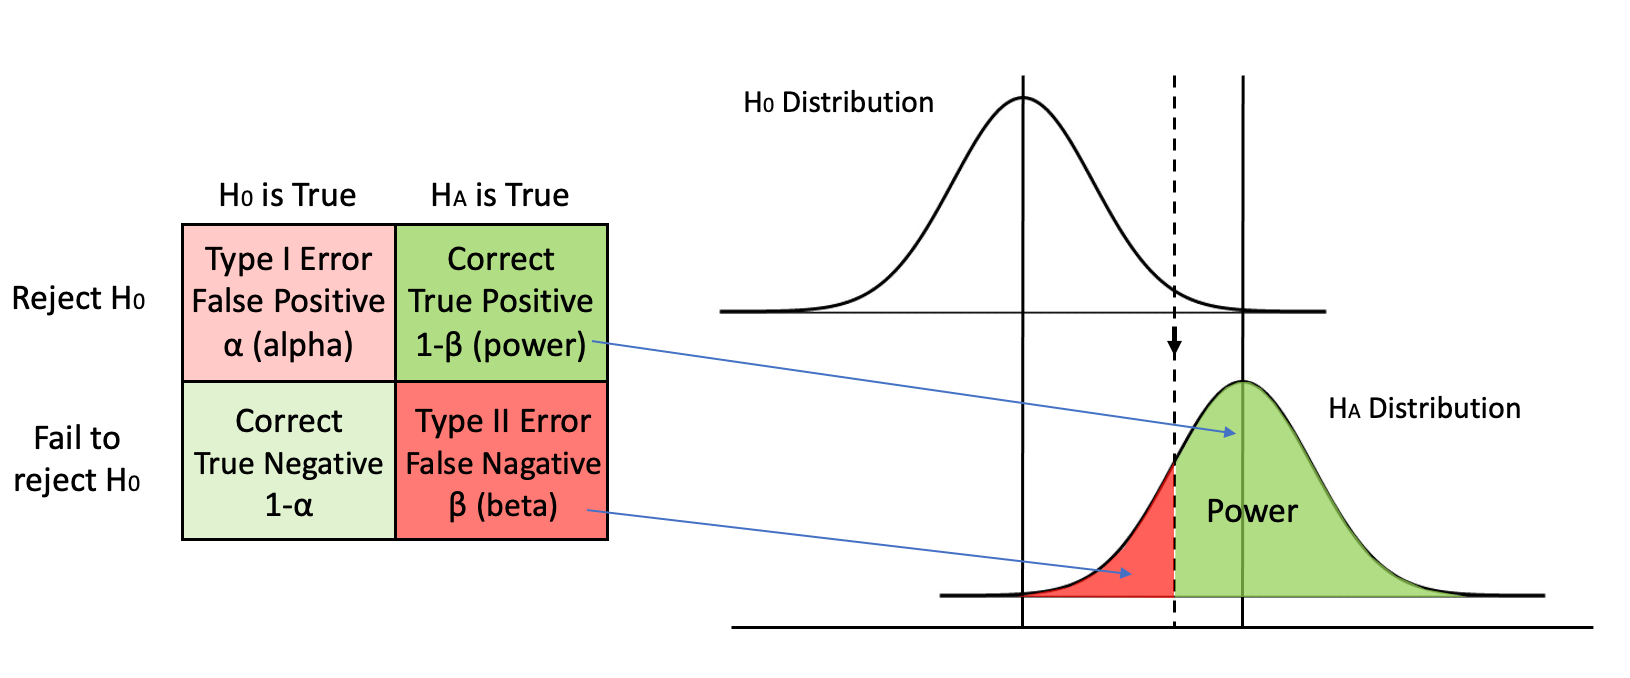
\includegraphics[width=1\textwidth]{../images/power.png}
	\onslide<2->{``But wait, shouldn't underpowered studies just lead to false negatives?''}
	\onslide<3->{``Underpowered studies are a major contributing factor to the reporting of both false positives and false negatives (Button et al., 2013).''
	
	i.e. ``winner's curse'' and ``file drawer problem''}

\end{frame}

\begin{frame}{Aside: Winner's Curse}
\begin{columns}
\column{0.55\textwidth}

	\begin{block}<1->{Winner's Curse}
		In an auction bid, the winner is the bidder making the highest estimate. If we assume that the average bid (before auction) is accurate, then the highest bidder overestimates the item's value. Thus, the auction's winner is likely to overpay. 
	\end{block}
	\column{0.45\textwidth}
	\includegraphics<1->[width=1\textwidth]{../images/bidding.jpg}
\end{columns}

\begin{exampleblock}<2->{Winner's Curse in Science}
	The term winner's curse is also used in statistics to refer to the regression toward the mean phenomenon, where the  the first person to report a significant test (the winner) will also report an effect size much larger than is likely to be seen in subsequent replication studies
\end{exampleblock}

\end{frame}

\begin{frame}{Aside: File-Drawer Problem}
	\begin{columns}
	\column{0.55\textwidth}
	
		\begin{block}<1->{File-Drawer Problem}
			Results not supporting the hypotheses of researchers often go no further than the researchers' file drawers, leading to a bias in published research.
		\end{block}
		\begin{exampleblock}<2->{Publication-Bias}
			Why? Because journals are biased to published \textbf{positive results} (3x more likely)

			This motivates researchers to manipulate their findings to ensure statistically significant results (either consciously or unconsicously)
		\end{exampleblock}
		\column{0.45\textwidth}
		\includegraphics<1->[width=1\textwidth]{../images/file-drawer.jpg}
	\end{columns}
	
\end{frame}

\begin{frame}{Back to the Incentives Paper}
	``Exploratory studies (i.e., those with low R) are much less likely to be true than confirmatory studies
		(i.e., those with high R) \textbf{even if the p-value generated is the same}, but arguably, current incentive
		studies reward novel (i.e., exploratory) findings over replication (i.e., confirmatory) studies.''

	\vspace{10pt}
	
	\onslide<2->Scientists have incentives to:
	\begin{itemize}
		\item<3-> publish in high-impact journals
		\item<4-> publish novel results (as opposed to trying to reproduce previous results)
		\item<5-> publish often (easier to publish if findings are positive)

	\end{itemize}
	
\end{frame}

\begin{frame}{Incentives: Maximising Fitness}
	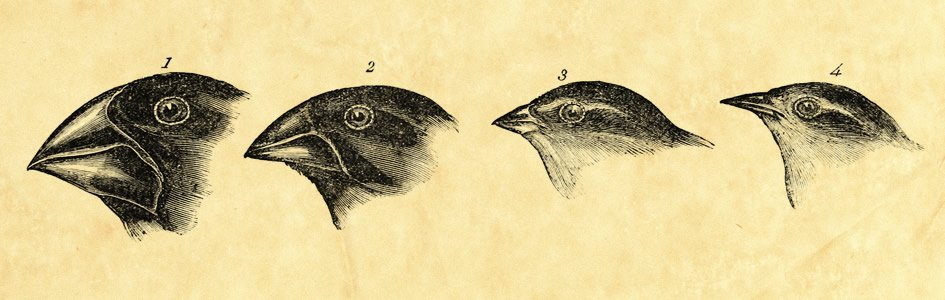
\includegraphics[width=1\textwidth]{../images/natural-selection.jpg}

	\begin{itemize}
		\item<1-> ``We used optimality theory to predict the rational strategy of a scientist possessing finite
		resources who seeks to maximise the career value of his or her publications.''
		\item<2-> ``We considered that researchers must choose how to divide their resources between exploratory studies that seek to
		identify new phenomena and confirmatory studies that attempt to verify previous findings
		and that they must decide the amount of resources to invest per study.''
	\end{itemize}
	
\end{frame}

\begin{frame}{Incentives: Results}
	\begin{textblock*}{300pt}(10pt,45pt)
		\begin{itemize}
			\item<1-> The current environment for scientists encourages publishing \textbf{novel} findings with \textbf{positive} results (which in turn encourages bad behaviour)
		\end{itemize}
	\end{textblock*}
	
	\begin{textblock*}{150pt}(210pt,100pt)
		\includegraphics<2->[width=1\textwidth]{../images/Netherlands_FalsifyData.png}
	\end{textblock*}

	\begin{textblock*}{150pt}(10pt,90pt)
		\includegraphics<3->[width=1\textwidth]{../images/HarvardProfFalsifyData.png}
	\end{textblock*}

	\begin{textblock*}{150pt}(100pt,150pt)
		\includegraphics<4->[width=1\textwidth]{../images/DukeProfessorFalsifyData.png}
	\end{textblock*}

	\begin{textblock*}{190pt}(100pt,110pt)
		\includegraphics<5->[width=1\textwidth]{../images/StanfordPresident.png}
	\end{textblock*}

\end{frame}

\begin{frame}{Incentives: Results}
	\begin{textblock*}{300pt}(10pt,45pt)
		\begin{itemize}
			\item<1-> This in turn results in approximately $50\%$ of publications likely to be false
		\end{itemize}
	\end{textblock*}
	
	\begin{textblock*}{120pt}(230pt,100pt)
		\includegraphics<2->[width=1\textwidth]{../images/25percentClinicalTrialsFalse.png}
	\end{textblock*}

	\begin{textblock*}{200pt}(10pt,80pt)
		\includegraphics<3->[width=1\textwidth]{../images/moststudiesfalse.png}
	\end{textblock*}

	\begin{textblock*}{220pt}(10pt,130pt)
		\begin{itemize}
			\item<4-> ``Open Science Collaboration reported that of 100 psychology studies selected from leading
			journals, only a minority of findings (approximately 40\%) could be replicated.''
			\item<5-> ``Similar results have been obtained by the pharmaceutical industry attempting to reproduce “landmark” findings from the published academic literature''
		\end{itemize}
	\end{textblock*}

	\begin{textblock*}{300pt}(30pt,50pt)
		\includegraphics<6->[width=1\textwidth]{../images/reproducible_neuroimaging.png}
	\end{textblock*}

\end{frame}

\begin{frame}{Incentives: Results}
	\begin{itemize}
		\item<1-> Competition for funding and prestige may also contribute to strategic-game playing [23]
		\item<2-> Current incentives that encourage scientists to build momentum around a single research focus may also be problematic [24]
		\item<3-> A survey of early career researchers indicated that ``survival mentoring'' (i.e., guidance on how to survive in the profession) is associated with 		increased odds of questionable behaviour in methods		
	\end{itemize}
\end{frame}


\begin{frame}{Incentives: Suggestions}
	\begin{itemize}
		\item<1-> Reduce incentives for novel findings (HOW?); 
		\item<2-> Emphasis should not be placed on a select number of publications for promotion
		\item<3-> Journals should be more stringent with statistics ($\alpha < 0.01$) and sample size (power)
	\end{itemize}

	\begin{alertblock}<4->{Note}
		I don't actually think these suggestions are all that great...
	\end{alertblock}
\end{frame}

\begin{frame}{Everything is F*cked}
	

	\begin{center}
	
\includegraphics[width=.7\textwidth]{../images/everything.png}
	\end{center}
	\begin{itemize}
		\item<2-> Week 2: Significance testing is f*cked
		\item<2-> Week 3: Causal inference from experiments is f*cked
		\item<2-> Week 5: Covariates are f*cked
		\item<2-> Week 6: Replicability is f*cked
		\item<2-> Week 8: Scientific publishing is f*cked
		\item<2-> Week 9: Meta-analysis is f*cked
		\item<2-> Week 10: The scientific profession is f*cked
	\end{itemize}

	\begin{textblock*}{300pt}(10pt,255pt)
		\tiny{\url{thehardestscience.com/2016/08/11/everything-is-fucked-the-syllabus/}}

	\end{textblock*}
\end{frame}

%%%%%%%%%%%%%%%
%% Publshing %%
%%%%%%%%%%%%%%%

\section{Publishing World}
\begin{frame}{Publishing World}
	Current state of the publishing world is:
	\begin{itemize}
		\item<2-> Lab A writes a paper, submits it to a for-profit* journal (owned by a small number of commercial publishers)
		\item<3-> Journal exports the labour of reviewing to scientists. For free.
		\item<4-> If manuscript is accepted, the Lab is billed hundreds to thousands of dollars (usually paid for by public grants)
		\item<5-> On top of this, the researcher often loses copyright to their articles, which the publisher subsequently can make money off in their subscription scheme
		\item<6-> Universities then have to pay to gain access.
		\item<7-> Finally: journal makes money... ``bigger profit margins than Google, Amazon and Apple''
	\end{itemize}
	
	\begin{textblock*}{300pt}(10pt,255pt)
		\onslide<2->{\tiny{*: usually}}
	
	\end{textblock*}
		
\end{frame}

\begin{frame}{Publishing World}
\begin{itemize}
	\item This has been called a triple payment system: \\``The government finances the research, pays salaries to those who carry out the quality control, and finally ends up buying the published product''
	\item<2-> The three biggest publishers in 2020 were Elsevier (18.1 per cent), Springer Nature (13 per cent), and Wiley (9.5 per cent). Their turnover was \$5.1 B, \$2.7 B and \$1.3 B CAD, respectively
	\item<3-> The profit margins for Elsevier was 37.9\%, and 27.9\% for Wiley (!!!)
	\item<4-> This is public money that could be spent on research
\end{itemize}
	
\end{frame}

\begin{frame}{Publishing World}
	In terms of open-access, things are getting better... 

\begin{center}
	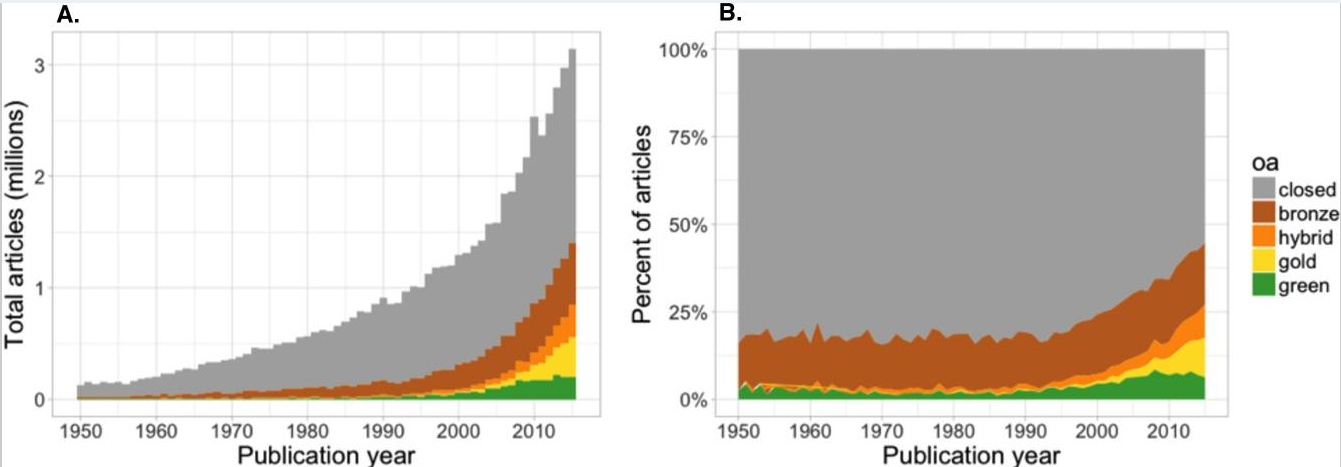
\includegraphics[width=.8\textwidth]{../images/openaccesstimeline.png}
\end{center}

	\vspace{-10pt}
	
	\footnotesize{
	\begin{itemize}

		\item<2-> Bronze: articles made free-to-read on the publisher website, without an explicit Open license
		\item<3-> Hybrid: articles are published in a subscription journal but are immediately free to read under an open license, in exchange for an article processing charge
		\item<4-> Gold: articles are published in an ``OA journal,'' a journal in which all articles are open directly on the journal website
		\item<5-> Green: Green articles are published in a toll-access journal, but self-archived in an OA archive (such as ArXiv preprint)
	\end{itemize}}

	\begin{textblock*}{300pt}(10pt,257pt)
		\tiny{https://www.ncbi.nlm.nih.gov/pmc/articles/PMC5815332/}
	
	\end{textblock*}

\end{frame}

\begin{frame}{Publishing World}
	\begin{textblock*}{300pt}(10pt,30pt)
		And people are taking things into their own hands\dots

	\end{textblock*}
	
	\begin{textblock*}{300pt}(10pt,50pt)
		\includegraphics<2->[width=.7\textwidth]{../images/NeuroImage_Resign.png}

	\end{textblock*}

	\begin{textblock*}{300pt}(140pt,100pt)
		\includegraphics<3->[width=.7\textwidth]{../images/scihub.png}

	\end{textblock*}

	
\end{frame}

%%%%%%%%%%%%
%% Grants %%
%%%%%%%%%%%%

\section{Grants}
\begin{frame}{Grants}

	85\% of investments in biomedical research is wasted (due to cumulative effects of bad production and reporting of research)$^{1}$

	\begin{itemize}
		\item<2-> We fund too few scientists: funding is largely concentrated in the hands of a few investigators
		\item<3-> We do not fund young investigators$^{2}$: 
		\begin{itemize}
			\item<4-> average age of biomedical scientists receiving their first substantial grant is 46 (and increasing) 
			\item<5-> the average age for a full professor in the U.S. is 55 (and growing)
			\item<6-> only 1.6 percent of funding in the NIH's Research Project Grant program went to principal investigators younger than 36 in 2017, but 13.2 percent went to those 66 and older.
		\end{itemize}
		\item<7-> We fund the wrong fields: well-funded fields attract more scientists to work for them, which increases their lobbying reach, fueling a vicious cycle. Allocation of bio-medical resources can be more strongly correlated to previous allocations and research than to BoD.
	\end{itemize}
	

	\begin{textblock*}{300pt}(10pt,250pt)
		\tiny{1: \url{thelancet.com/journals/laneur/article/PIIS1474-4422(19)30481-8/fulltext}\\ 2: \url{scientificamerican.com/article/science-funding-is-broken/}}

	\end{textblock*}
	
\end{frame}

\begin{frame}{Grants}
	\begin{itemize}
		\item We do not spend enough: in many countries, public funding has stagnated and is under increasing threat from contesting budget items
	\end{itemize}
	
	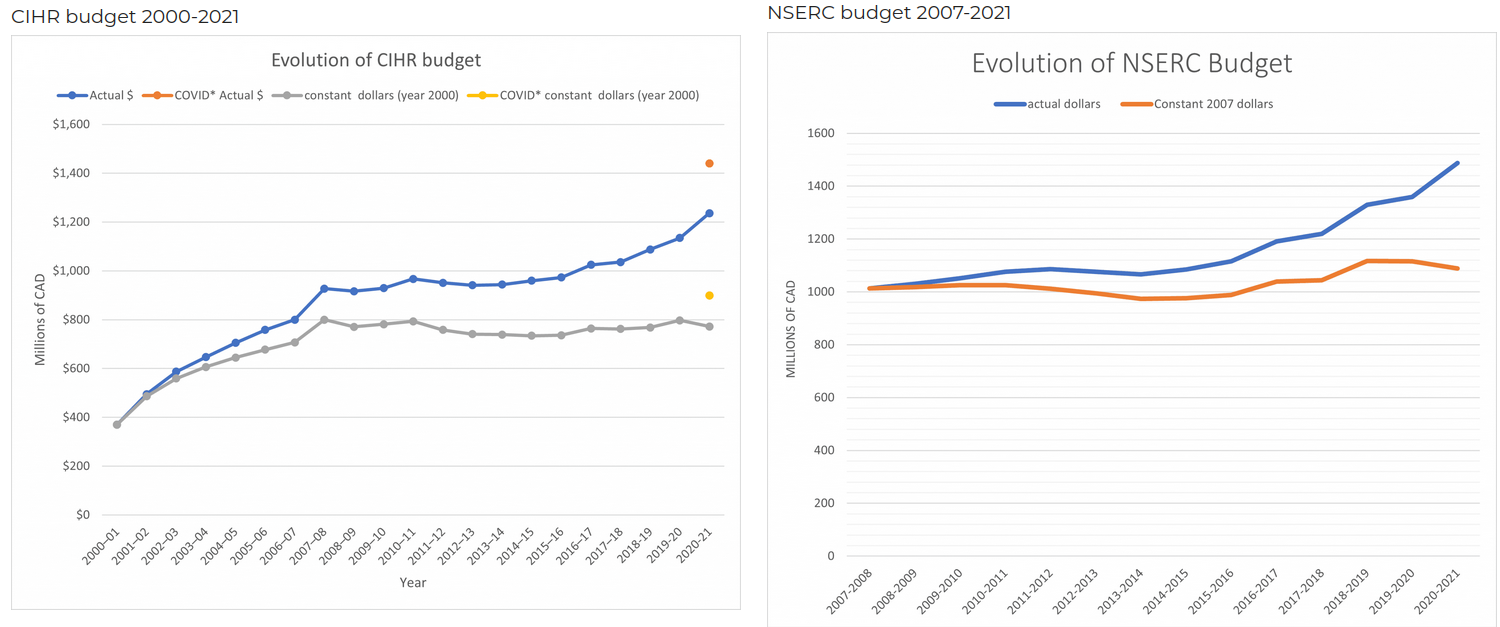
\includegraphics[width=1\textwidth]{../images/grantsCanada.png}

	\begin{textblock*}{300pt}(10pt,240pt)
		\tiny{https://can-acn.org/science-funding-in-canada-statistics/}

	\end{textblock*}
\end{frame}

\begin{frame}{Grants}
	This problem is especially bad in Canada:

	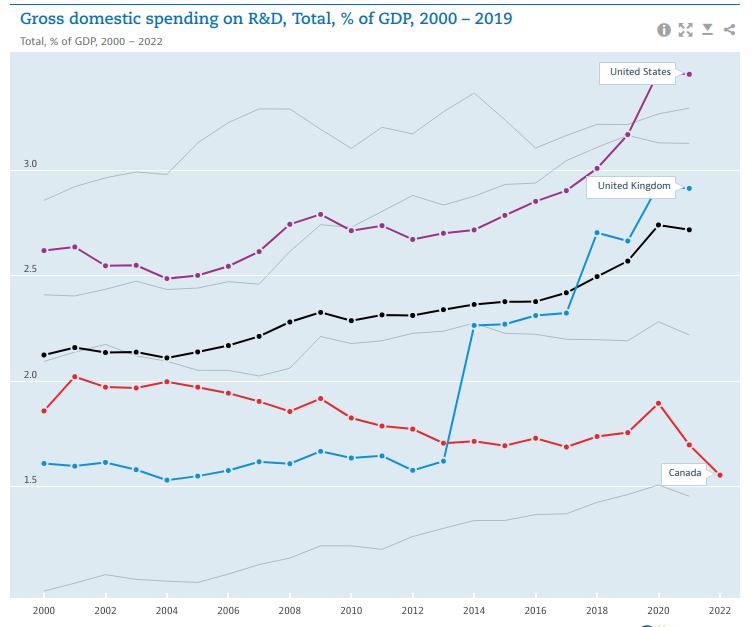
\includegraphics[width=.7\textwidth]{../images/fundinggdpcountries.png}

	\begin{textblock*}{300pt}(10pt,250pt)
		\tiny{https://can-acn.org/science-funding-in-canada-statistics/}

	\end{textblock*}
\end{frame}

\begin{frame}{Grants}
	\begin{itemize}
		\item<1-> We reward big spenders: hiring, promotion and tenure often rest on the researcher's ability to secure high levels of funding. But expenses do not necessarily correlate with importance
		\item<2-> We do not fund high-risk ideas: the pressure that taxpayer money be “well spent” leads government funders to back projects most likely to pay off with a `positive result'
	\end{itemize}

	\vspace{10pt}

	\onslide<3->More on these ideas when we get to metascience...
\end{frame}

%%%%%%%%%%%%%%%%%%%
%% Grad Students %%
%%%%%%%%%%%%%%%%%%%

\section{Grad Students}
\begin{frame}{Grad Students}
	Funding for grad students is well below the poverty line
	
	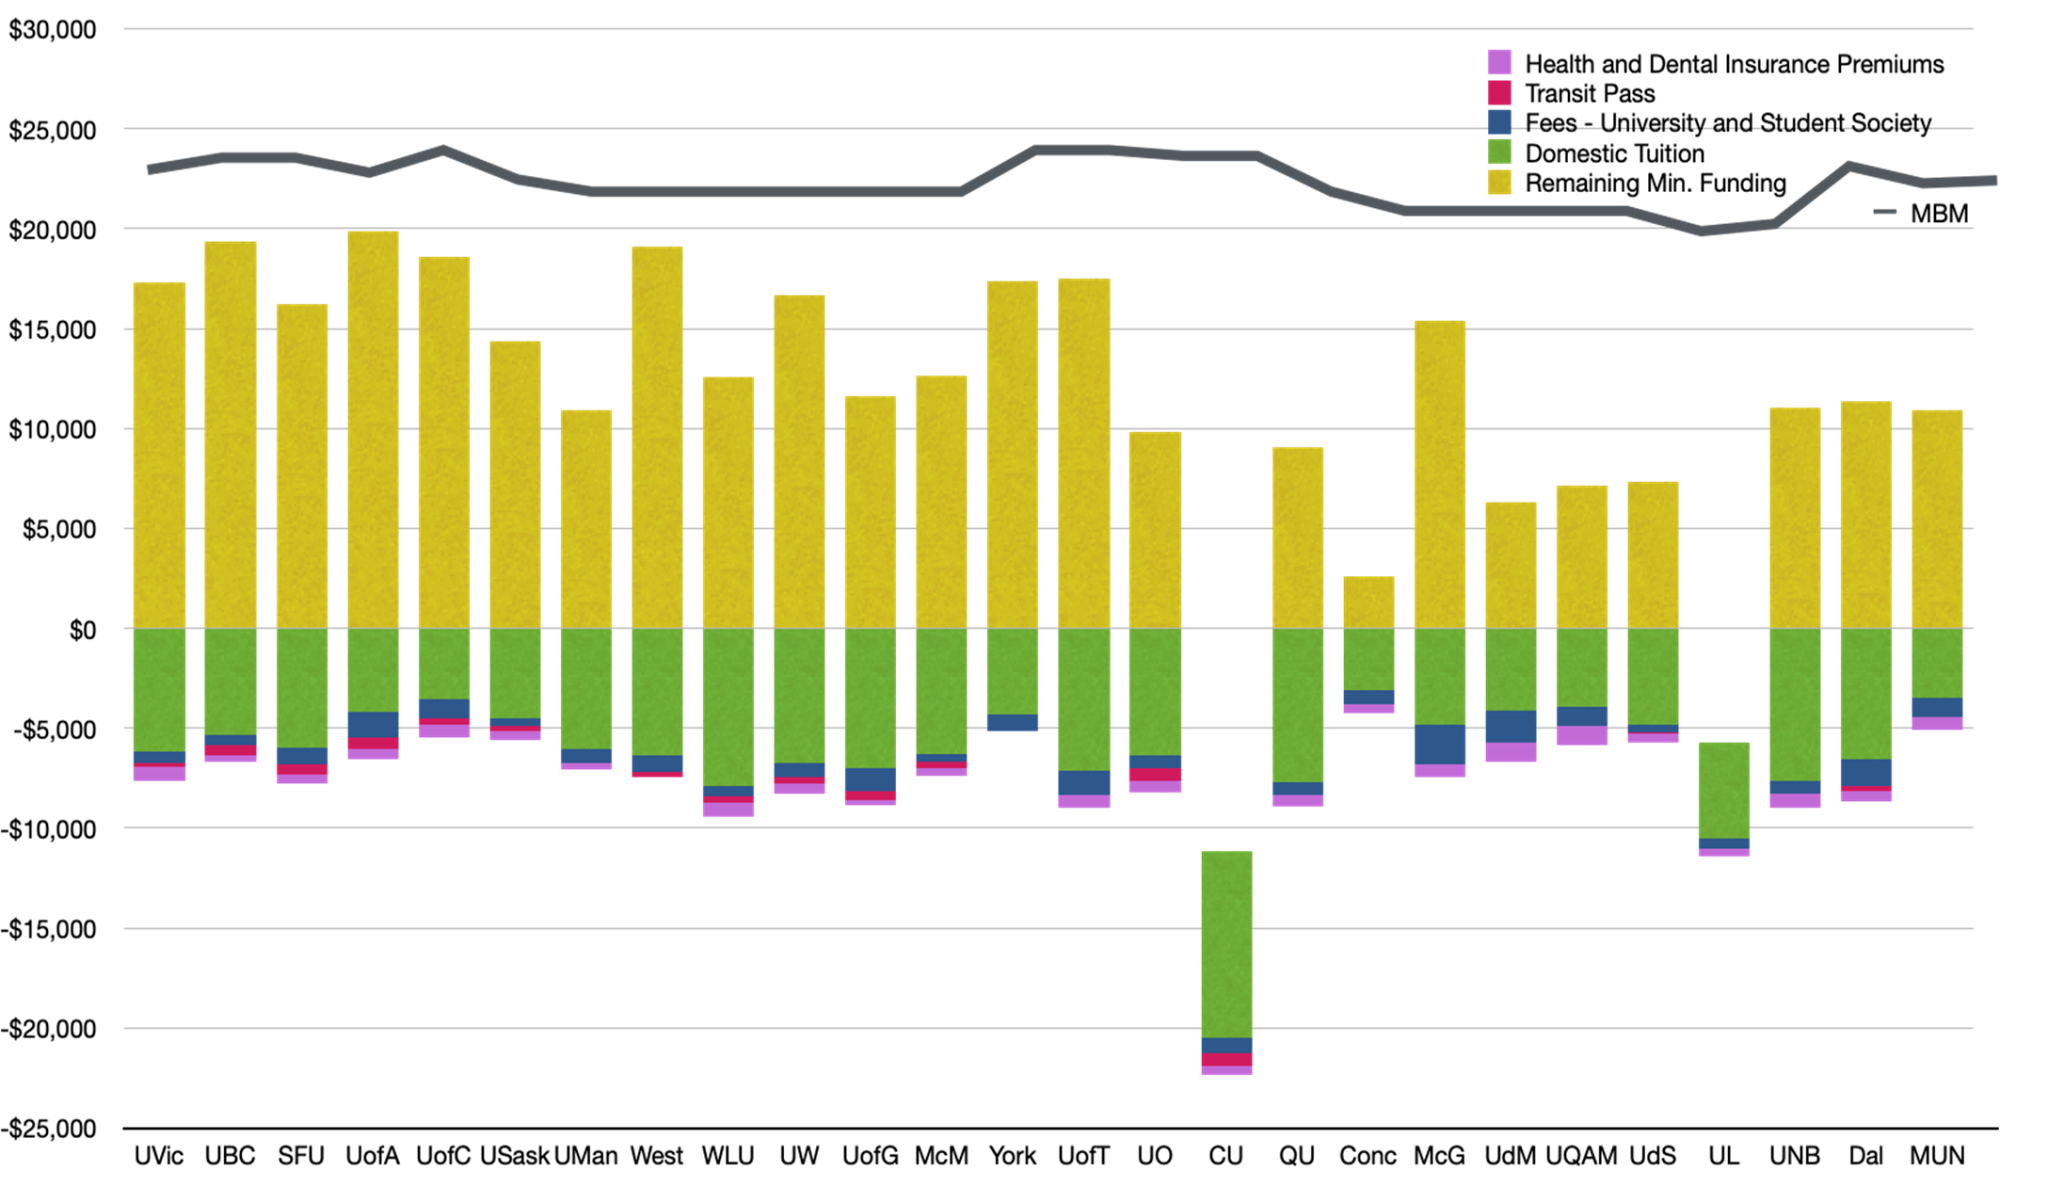
\includegraphics[width=1\textwidth]{../images/gradfundpovertyline.png}
	
	\tiny{https://www.universityaffairs.ca/career-advice/career-advice-article/the-high-cost-of-inadequate-funding-for-grad-students/}

\end{frame}

\begin{frame}{Grad Students}
	\begin{columns}
	\column{0.35\textwidth}

	This situation is even worse when you take into account the cost of living in those cities

	\column{0.65\textwidth}
	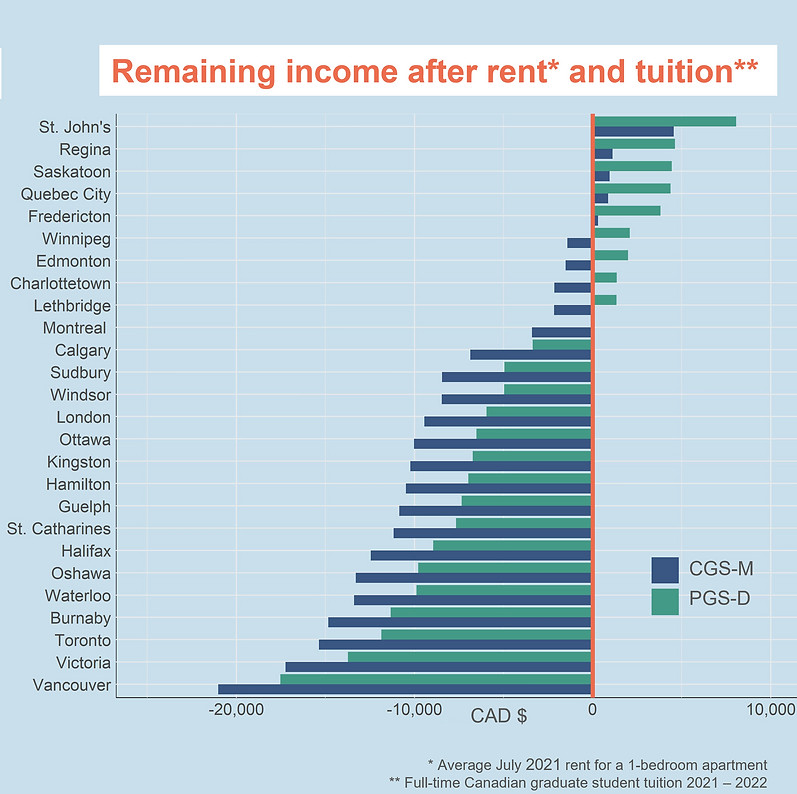
\includegraphics[width=1\textwidth]{../images/gradmoneyafterrent.jpeg}

	\tiny{https://www.supportourscience.ca/learn-more}
	\end{columns}
\end{frame}

\begin{frame}{Grad students}
	\begin{columns}
		\column{0.65\textwidth}
		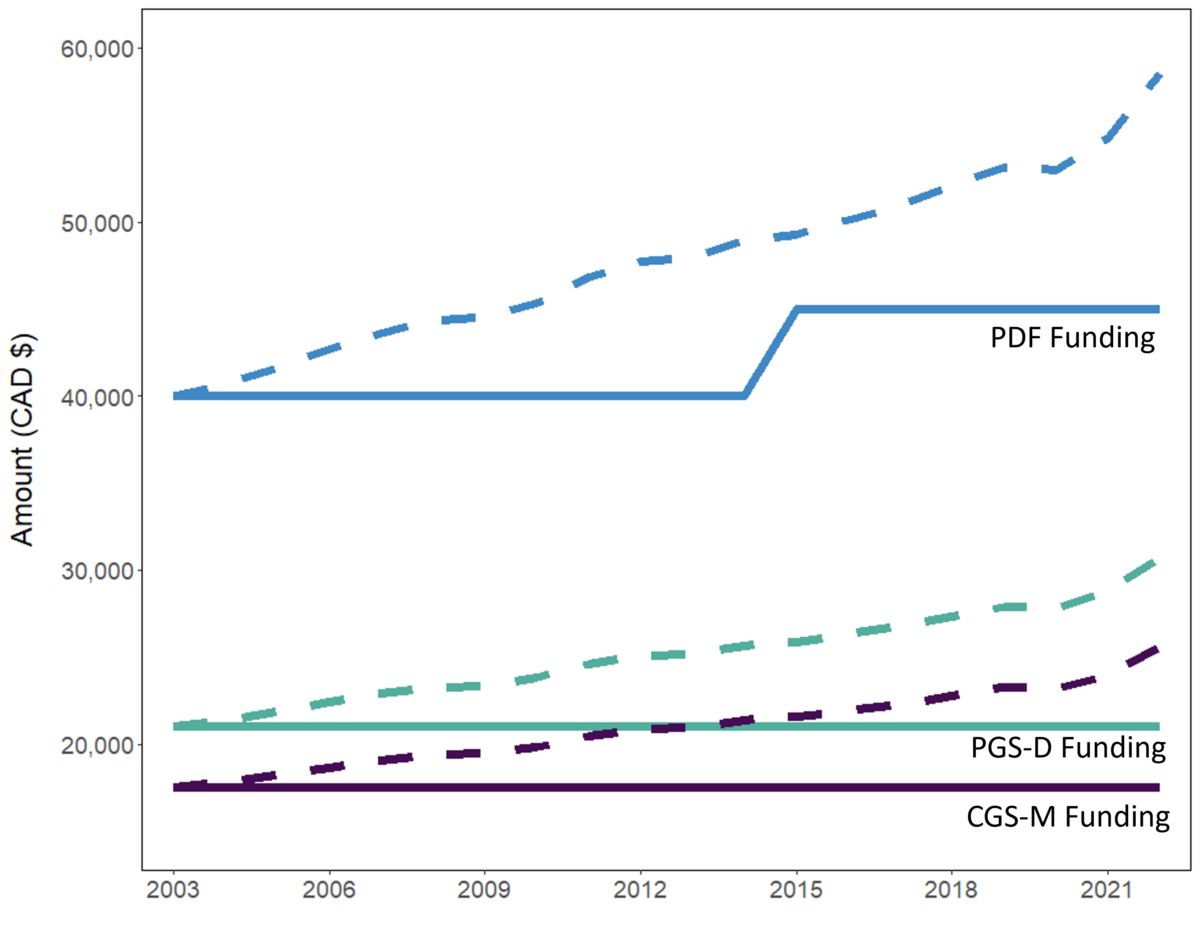
\includegraphics[width=1\textwidth]{../images/gradfundingtime.png}
		\tiny{https://www.supportourscience.ca/learn-more}
		\column{0.35\textwidth}
		Graduate student scholarship (CGS-M \& PGS-D) and postdoctoral scholar fellowship (PDF) award amounts have not kept pace with inflation (dashed lines) in Canada. Data available in the Support Our Science Data Repository.
	\end{columns}
\end{frame}

\begin{frame}{Grad Students}
	\begin{columns}
		\column{0.55\textwidth}
		It gets worse. The number of graduate scholarships (CGS-M, PGS-D, CGS-D) decreased in 2010, and has remained relatively steady since. However, in that same time period graduate student enrollment in Canada has doubled.
		\column{0.45\textwidth}
		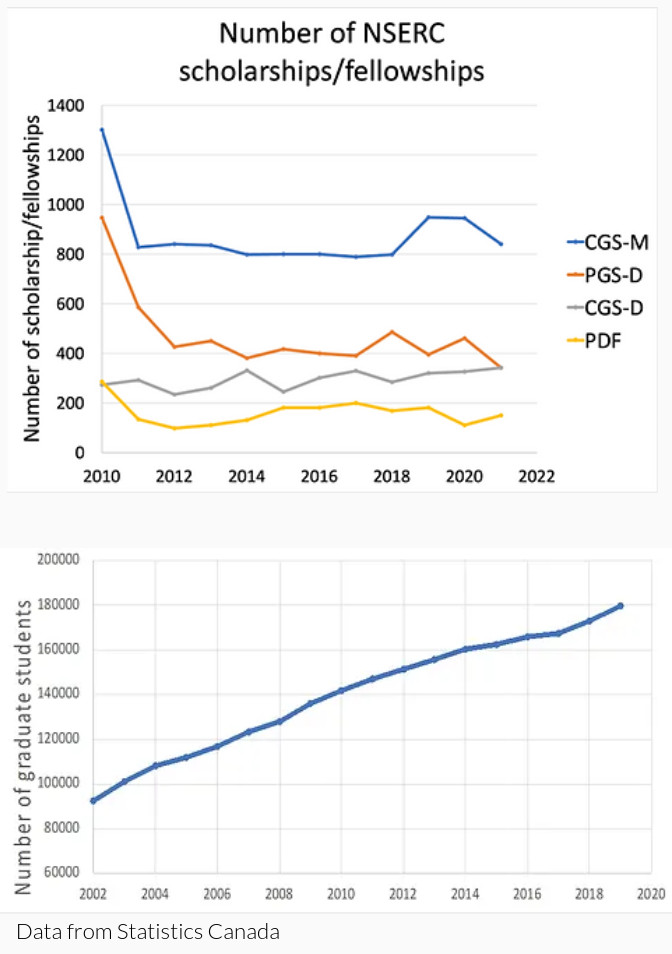
\includegraphics[width=1\textwidth]{../images/gradnumberscholarships.jpeg}
	\end{columns}
	
\end{frame}

\begin{frame}{Grad students}
	Is academia a pyramid scheme? ``The number of PhD graduates in Canada is growing while the
	number of open tenure-track positions is stagnant or declining''

	\begin{flushright}
		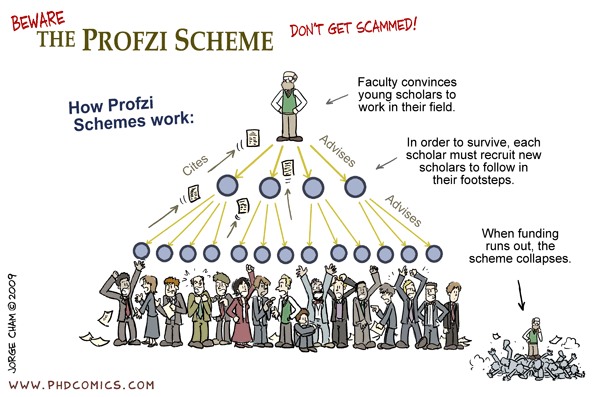
\includegraphics[width=0.7\textwidth]{../images/pyramidscheme}		
	\end{flushright}


Counter: these students gain skills that serve them well in other careers
\end{frame}

\begin{frame}{Grad Students}
	But does getting a MSc or PhD even set you up for success?
	
	\begin{itemize}
		\item<2-> On the one hand, PhD graduates experience lower levels of unemployment
		and higher earnings than graduates with master's or bachelor's degrees. 
		\item<3-> On the other hand: ``For men with PhDs working full-time, the economic return of a PhD over a
		master's degree has been declining; furthermore, the return is lower and
		dropping more quickly for those under 40 years of age. In contrast, for women
		with PhDs working full-time, the economic return has been rising for the overall
		population and for those under 40. Having said this, the earnings of men are still
		considerably higher than those of women overall. ''
	\end{itemize}

\end{frame}

\begin{frame}{Grad Students}
	What about mental health?

	\begin{itemize}
		\item<2-> Graduate students are around two to six times more likely to experience depression and anxiety than the general population$^{1}$
		\item<3-> Mental health is the major factor behind the high attrition rates in PhD programs.
	\end{itemize}

	\onslide<4->{What are the causes?}
	\begin{itemize}
		\item<5-> work-family interface, 
		\item<6-> job demands and job control, 
		\item<7-> the supervisor's leadership style, 
		\item<8-> team decision-making culture, 
		\item<9-> and perception of a career outside academia$^{2}$
	\end{itemize}

	\begin{textblock*}{300pt}(10pt,240pt)
		\tiny{1: \url{https://www.nature.com/articles/s41587-019-0179-y} \\ 2: \url{https://www.sciencedirect.com/science/article/abs/pii/S0048733317300422}}

	\end{textblock*}
\end{frame}

%%%%%%%%%%%%%%%%%
%% Philosophy of Science %%
%%%%%%%%%%%%%%%%%

\section{Philosophy of Science}

\begin{frame}{Philosophy of Science}
	\begin{textblock*}{150pt}(10pt,50pt)
		\includegraphics<1->[width=1\textwidth]{../images/The_Scientific_Method.png}

	\end{textblock*}

	\begin{textblock*}{150pt}(200pt,75pt)
		\includegraphics<2->[width=1\textwidth]{../images/scienceprogress.png}

	\end{textblock*}

	\begin{textblock*}{300pt}(10pt,200pt)
		\begin{center}
			\onslide<3->{But does science work this way?}	
		\end{center}
	\end{textblock*}
\end{frame}

\begin{frame}{Philosophy of Science}

	\begin{textblock*}{50pt}(300pt,10pt)
		\includegraphics<2->[width=1\textwidth]{../images/comte.jpg}
	\end{textblock*}

	A brief history of \textbf{Philosophy of Science}:
	
	\vspace{10pt}
	
		\onslide<2->{Auguste Comte (1798-1857):}
		\begin{itemize}
			\item<3-> true nature is unknowable; 
			\item<4-> distrusted scientific explanations; 
			\item<5-> \textbf{Positivism}: observations should be recorded and from those observations, predictions can be made about what will be observed in the future
		\end{itemize}
		\onslide<6->{Vienna Circle (1920s and 30s):}
		\begin{itemize}
			\item<7-> went further than Comte: a statement was only meaningful if it had the potential to be observed/verified (called \textbf{Logical Positivism})
			\item<8-> However, critics say that logical positivism is self-refuting (itself can't be verified)
		\end{itemize}
	
\end{frame}

\begin{frame}{Philosophy of Science}

	\begin{textblock*}{50pt}(300pt,10pt)
		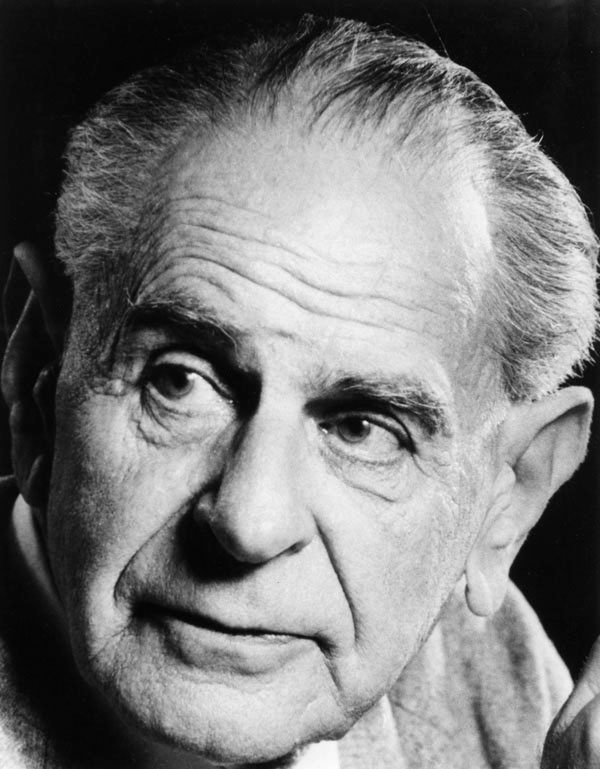
\includegraphics[width=1\textwidth]{../images/Karl_Popper.jpg}
	\end{textblock*}

	Karl Popper (1902-1994):
	\begin{itemize}
		\item<2-> Another problem with logical positivism can be seen \\ with the statement ``all swans are white''
		\item<3-> When can you say that you've proven a proposition?
		\item<4-> \textbf{Falsification}: theories should be constructed so that it is possible for an observation to prove them false
		\item<5->  i.e. a single observation which falsifies a theory should lead to that theory being abandoned
	\end{itemize}

	\onslide<6->{But does science work this way?}
	\begin{itemize}
		\item<7-> Isaac Newton's theory of gravitation was refuted almost immediately by the observed motion of the Moon. However, this evidence was cheerfully ignored and Newton's theories went on to very fruitfully dominate science for over two hundred years.
		\item<8-> Dark matter can be seen as a reluctance to reject our current model of the universe
	\end{itemize}

\end{frame}

\begin{frame}{Philosophy of Science}
	\begin{textblock*}{50pt}(300pt,10pt)
		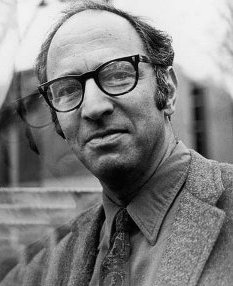
\includegraphics[width=1\textwidth]{../images/Thomas_Kuhn.jpg}
	\end{textblock*}
	Thomas Kuhn (1922-1996):
		\begin{itemize}
			\item<2-> in his `The Structure of Scientific Revolutions', Kuhn \\introduced the idea of \textbf{paradigm shifts}. Scientists \\operate within a paradigm until a scientific revolution leads to a fundamental shift (e.g. oxygen vs phlogistin; copernican revolution; quantum mechanics)
			\item<3-> once a paradigm is established, scientists perform `normal science': scientists work to solve puzzles and anomalies within the existing paradigm; progress is incremental
			\item<4-> then, anomalies and problems that cannot be explained within the current paradigm begin to accumulate, which can lead to a crisis (overwhelming contrary evidence)
			\item<5-> In response to a crisis, a revolutionary phase ensues, marked by the abandonment of the old paradigm and the emergence of a new one. This shift is often accompanied by a change in fundamental assumptions and a reevaluation of previously accepted scientific beliefs
		\end{itemize}

\end{frame}

\begin{frame}{Philosophy of Science}
	\begin{center}
		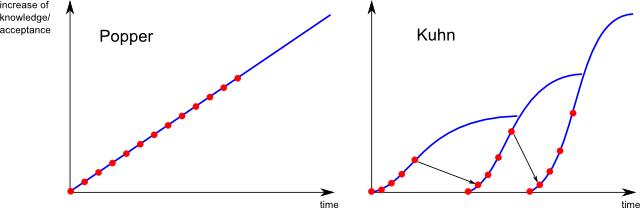
\includegraphics[width=1\textwidth]{../images/popper-kuhn1.png}
	\end{center}
\end{frame}

\begin{frame}{Philosophy of Science}
	\begin{textblock*}{50pt}(300pt,5pt)
		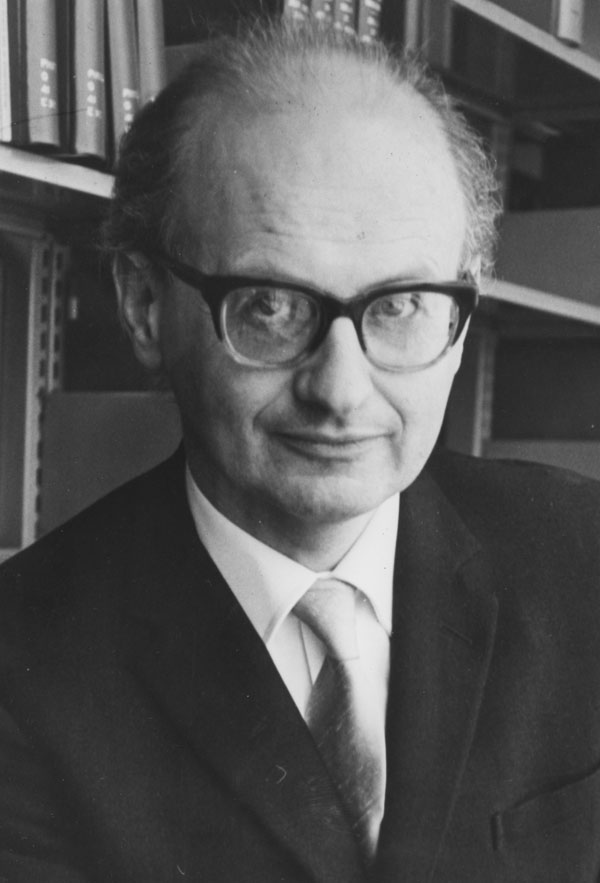
\includegraphics[width=1\textwidth]{../images/lakatos.jpg}
	\end{textblock*}
	Imre Lakatos (1922-1974):
		\begin{itemize}
			\item<2-> basic unit of science is the \textbf{research programme} \\ (e.g. Newtonian science; or quantum physics)
			\item<3-> a research programme consists of a core of central hypotheses which are rarely falsified, surrounded and protected by a band of secondary hypotheses which can be falsified. 
			\item<4-> If a central hypothesis is threatened by new evidence, then rather than chuck out the entire research programme, scientists tend to invent a `rescue hypothesis' to explain away the new findings. 
			\item<5-> Young, vigorous research programmes make predictions, said Lakatos, but eventually they become `degenerate': they no longer generate predictions and their adherents spend most of their efforts trying to defend the programme's core theses against mountains of contrary evidence
			\item<6-> Essentially, Lakatos is a more \textit{nuanced} take on Kuhn
		\end{itemize}

\end{frame}

\begin{frame}{Philosophy of Science}
\begin{center}
	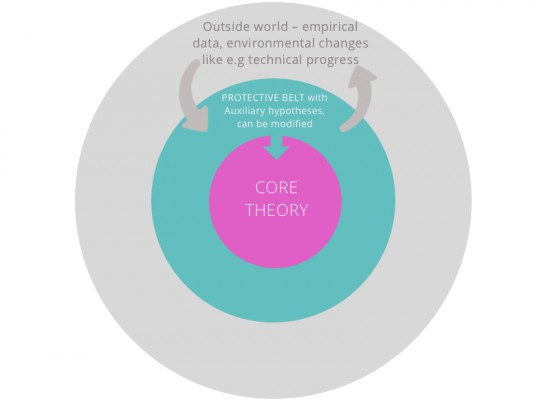
\includegraphics[width=.9\textwidth]{../images/lakatosmodel.jpg}
\end{center}
\end{frame}

\begin{frame}{Philosophy of Science}
	\begin{textblock*}{50pt}(300pt,10pt)
		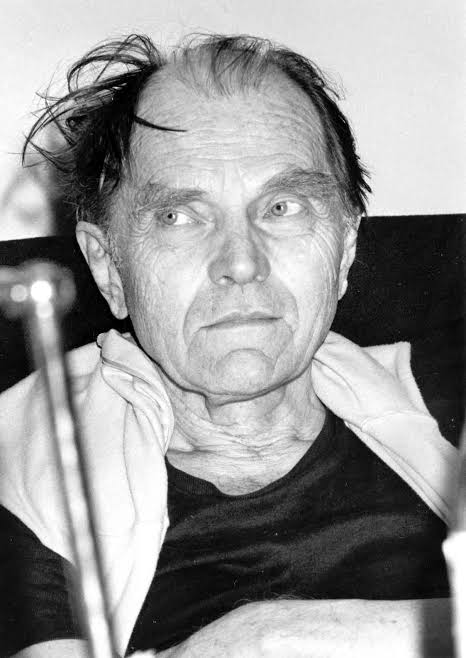
\includegraphics[width=1\textwidth]{../images/Feyerabend.jpeg}
	\end{textblock*}
	Paul Feyerabend (1924-1994):
		\begin{itemize}
			\item<2-> in his book `Against Method', Paul challenges the idea \\of a universal scientific method and argues for \\methodological pluralism. He does so with some\\ examples from the history of science:
			\begin{itemize}
				\item<3-> Copernican revolution: the Heliocentric model's success was not solely due to the use of a particular, universally accepted method. Instead, it involved a combination of empirical observations, persuasive rhetoric, and strategic maneuvering. 
				\item<4-> Galileo's hypothesis that the earth rotates on its axis employed a combination of empirical observations, rhetorical strategies, and even thought experiments to make his case
			\end{itemize}
			\item<5-> These episodes violated all common prescriptive rules of science. Feyerabend argues that applying such rules in these historical situations would actually have prevented scientific revolution.
		\end{itemize}
	
\end{frame}

\begin{frame}{Philosophy of Science}
	More examples of unconventional discoveries in the history of science:
	\begin{itemize}
		\item<2-> Penicillin (1928): Alexander Fleming left a petri dish open while he went on vacation. Later found that mold (Penicillium) had contaminated the dish, inhibiting bacterial growth
		\item<3-> X-rays (1895): Wilhelm Roentgen accidentally discovered while playing with cathode-ray tubes
		\item<4-> Microwave Oven (1945): candy bar in Percy Spencer's pocket melted when he stood too close to a magnetron
		\item<5-> Viagra (1990s): developed for hypertension and angina, during clinical trials they noticed male participants reporting improved erectile function
		\item<6-> Phosphorus (1669): Hennig Brand was attempting to create the philosopher's stone by boiling his own urine. Brand noticed that a white substance glowed in the dark and emitted a faint light. This discovery was unintentional and occurred as a byproduct of his alchemical experiments.
	\end{itemize}
\end{frame}

%%%%%%%%%%%%%%%%%
%% Metascience %%
%%%%%%%%%%%%%%%%%

\section{Metascience}
\begin{frame}{Metascience}
	\begin{block}{Metascience}
		The use of scientific methodology to study science itself. Metascience seeks to increase the quality of scientific research while reducing inefficiency
	\end{block}

	\begin{columns}
		\column{0.7\textwidth}
		\onslide<2->{``Science is the best thing that has happened to human beings \dots \\ but we can do it better.'' \\- John Ioannidis}
		\column{0.3\textwidth}
		\begin{center}
		\includegraphics<2->[width=.7\textwidth]{../images/John_Ioannidis.jpg}
		\end{center}
	\end{columns}
\end{frame}

\begin{frame}{Metascience}
	\begin{itemize}
		\item<1-> In 1966, an early meta-research paper examined the statistical methods of 295 papers published in ten high-profile medical journals. It found that, ``in almost 73\% of the reports read ... conclusions were drawn when the justification for these conclusions was invalid.''
		\item<2-> In 2005, John Ioannidis published a paper which argued that a majority of papers in the medical field produce conclusions that are wrong.\\
		\item[]<2-> 
\includegraphics[width=.7\textwidth]{../images/moststudiesfalse.png}
		\item<3-> Later meta-research identified widespread difficulty in replicating results in many scientific fields, including psychology and medicine. This problem was termed ``the replication crisis''
	\end{itemize}
\end{frame}

\begin{frame}{Metascience}
	Metascience can be categorized into five major areas of interest: 
	\begin{enumerate}
		\item<2-> Methods (how to perform)
		\item<3-> Reporting (how to communicate)
		\item<4-> Reproducibility (how to verify)
		\item<5-> Evaluation (how to evaluate)
		\item<6-> Incentives (how to reward research)
	\end{enumerate}
\end{frame}

\begin{frame}{Metascience}
	Methods examples:
	\begin{itemize}
		\item<2-> biases in research
		\item<3-> poor study design
		\item<4-> abuse of statistics (p-hacking)
	\end{itemize}
	\begin{block}<5->{p-hacking}
		Researchers collect or select data or statistical analyses until non-significant results become significant.
	\end{block}

	\onslide<6->{Reporting:}
	\begin{itemize}
		\item<7-> poor practices in reporting, explaining, disseminating and popularizing research
		\item<8-> reduces public's confidence in science
		\item<9-> solutions include the implementation of reporting standards, and greater transparency in scientific studies (conflict of interest)
	\end{itemize}
\end{frame}

\begin{frame}{Metascience}
	Reproducibility:
	\begin{itemize}
		\item<2-> Replication is an essential part of the scientific process, and the widespread failure of replication puts into question the reliability of affected fields.
		\item<3-> Replication of research (or failure to replicate) is considered less influential than original research, and is less likely to be published in many fields. This discourages the reporting of, and even attempts to replicate, studies.
	\end{itemize}
	\onslide<4->{Evaluation (i.e. quality and validity of scientific research):}
	\begin{itemize}
		\item<5-> Peer review (often blind and non-transparent)
		\item<6-> Quality of meta-analyses and systematic reviews: assessing potential biases, and providing recommendations for improving the methodology of these synthesis efforts
		\item<7-> Way more than I can fit in this slide \dots
\end{itemize}
\end{frame}

\begin{frame}{Metascience}
	Incentives:
	\begin{itemize}
		\item Critics argue that perverse incentives have created a publish-or-perish environment in academia which promotes the production of junk science, low quality research, and false positives.
		\item ``the number of publications has ceased to be a good metric as a result of longer author lists, shorter papers, and surging publication numbers''
		\item using number of publications, citation number, or impact factor can lead to: ``overproduction, unnecessary fragmentations, overselling, predatory journals (pay and publish), clever plagiarism, and deliberate obfuscation of scientific results so as to sell and oversell''
	\end{itemize}
\end{frame}

\begin{frame}{Metascience}

	\begin{columns}
		\column{0.3\textwidth}
		Is science stagnating?
		\column{0.7\textwidth}
		
\includegraphics[width=1\textwidth]{../images/stagnant.png}
	\end{columns}
	
	\begin{block}<2->{CD index}
		If a paper or patent is disruptive, the subsequent work that cites it is less likely to also cite its predecessors; for future researchers, the ideas that went into its production are less relevant (for example, Pauling's triple helix)
	\end{block}

	
\end{frame}

\begin{frame}{Metascience}
	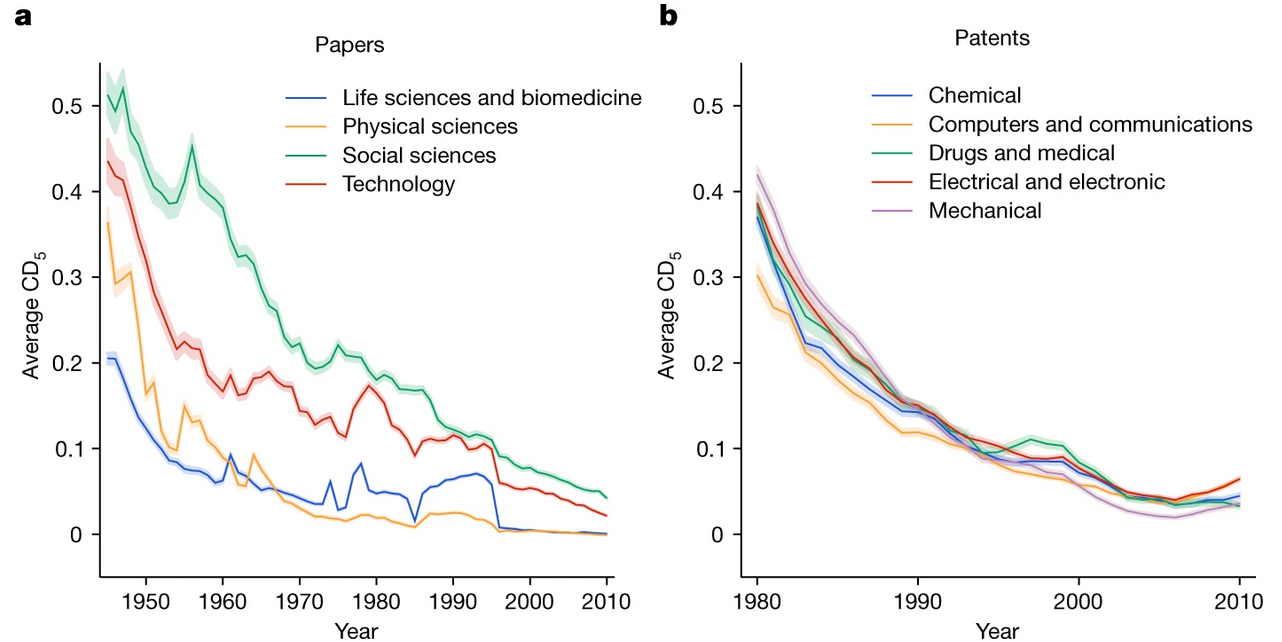
\includegraphics[width=1\textwidth]{../images/paperspatents.png}
\end{frame}

%%%%%%%%%%%%%%%
%% Solutions %%
%%%%%%%%%%%%%%%

\section{Solutions}

\begin{frame}{Solutions}

	\begin{itemize}
		\item Pre-register your study (publish all well-designed studies, regardless of results; less chance for p-hacking)
		\item<2-> Scientists' advancement should be based not only on their discoveries but also on their replication track record (encourage replication)
		\item<3-> Publish in open-access (preferably non-profit) journals (the public funds research; there should be no gatekeeping)
		\item<4-> Ensure your ethics allows you to publish your data; then publish your data and code (allows researchers to better check findings) 
		\item<5-> Use a lottery to decide which grant applications to fund (perhaps after they pass a basic review; we don't necessarily know what will result in the best science - introduce more randomness)
		\item<6-> Shift funding from senior people to younger researchers (even in the same lab; the average age of biomedical scientists receiving their first substantial grant is 46 and is increasing over time)
	\end{itemize}
	
\end{frame}

\begin{frame}{More Solutions}

	\begin{itemize}
		\item More funds should be earmarked for new fields and fields that are high risk (again, we don't actually know what the next big breakthrough will be)
		\item<2-> Quit our dependence on p-value. Confidence intervals, effect sizes, Bayesian methods, etc.
		\item<3-> Researchers should be encouraged to switch fields, whereas currently they are incentivized to focus in one area
		\item<4-> We should invest in studying how to get the best science and how to choose and reward the best scientists. We should not trust opinion (including my own) without evidence. This will improve public opinion and hopefully funding!
	\end{itemize}
	
\end{frame}

\begin{frame}{Summary}
	\begin{itemize}
		\item Our incentive structure (publish or perish) leads to many publications that cannot be reproduced
		\item<2-> The publishing industry wastes money and needs to be improved (more rigorous stats; publish negative findings; publish papers trying to reproduce other studies )
		\item<3-> We tend to fund the wrong kind of research (too safe) and the wrong people (senior academics)
		\item<4-> Grad students are not paid enough and are not being trained for the realistic job landscape they will enter
		\item<5-> Science doesn't necessarily work the way we might think
		\item<6-> Metascience - the science of science - can help us improve how we do good science
	\end{itemize}
	
\end{frame}

\begin{frame}{Further Reading}
	\begin{textblock*}{60pt}(10pt,30pt)
		
\includegraphics[width=1\textwidth]{../images/statsdonewrong.jpg}
	\end{textblock*}

	\begin{textblock*}{60pt}(80pt,30pt)
		
\includegraphics[width=1\textwidth]{../images/againstmethod.jpg}
	\end{textblock*}

	\begin{textblock*}{60pt}(150pt,30pt)
		
\includegraphics[width=1\textwidth]{../images/structures.jpg}
	\end{textblock*}

	\begin{textblock*}{60pt}(220pt,45pt)
		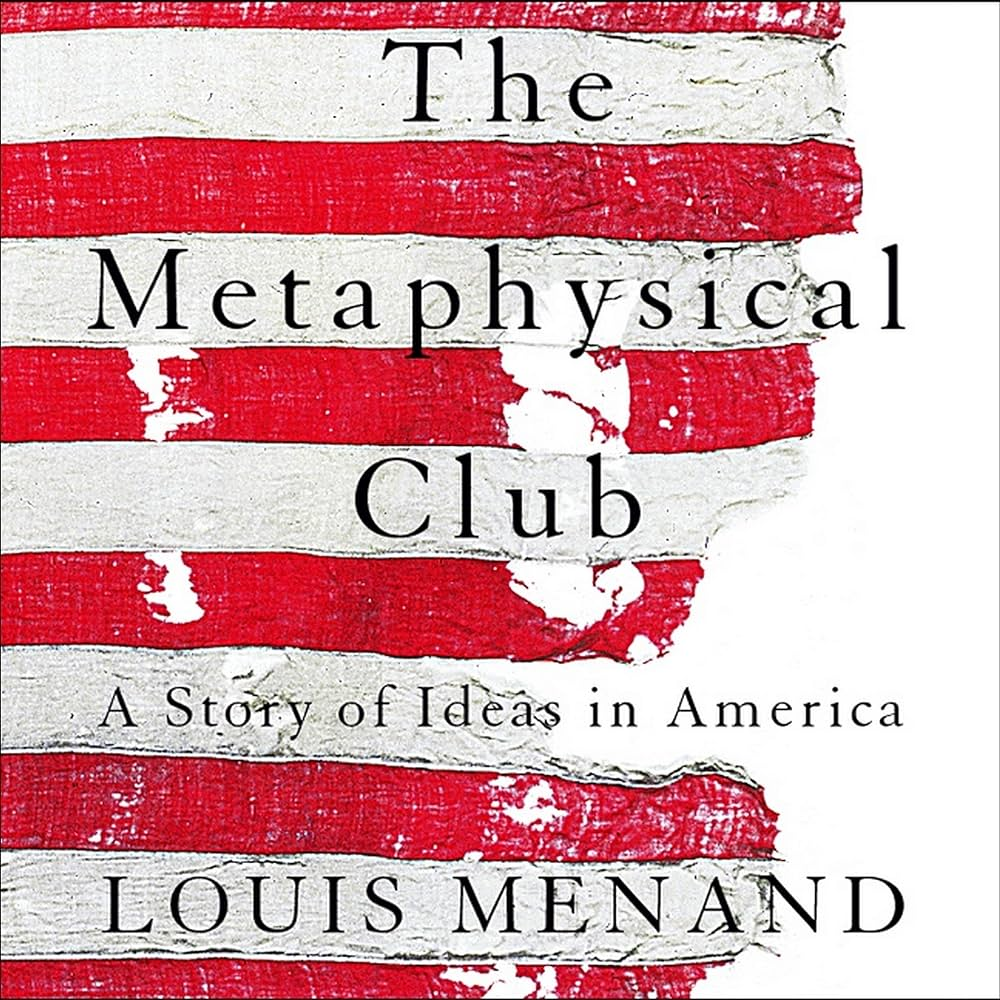
\includegraphics[width=1\textwidth]{../images/metaphysicalclub.jpg}
	\end{textblock*}

	\begin{textblock*}{60pt}(290pt,30pt)
		
\includegraphics[width=1\textwidth]{../images/degreesofsuccess.png}
	\end{textblock*}

	\begin{textblock*}{190pt}(10pt,130pt)
		
\includegraphics[width=1\textwidth]{../images/moststudiesfalse.png}
	\end{textblock*}

	\begin{textblock*}{160pt}(200pt, 130pt)
		
\includegraphics[width=1\textwidth]{../images/sciencefunding.png}
	\end{textblock*}

	\begin{textblock*}{80pt}(60pt,175pt)
		
\includegraphics[width=1\textwidth]{../images/25percentClinicalTrialsFalse.png}
	\end{textblock*}

	\begin{textblock*}{200pt}(175pt,190pt)
		This talk can be downloaded from: \url{https://github.com/WeberLab/MetascienceTalk}\\
		You can find me on Mastodon: \href{https://qoto.org/@weberam2}{@weberam2@qoto.org}
	\end{textblock*}

\end{frame}

\end{document}
